\documentclass[a4paper,12pt]{report}

\usepackage[utf8]{inputenc}
\usepackage{graphicx}
\usepackage{float}
\usepackage{hyperref}
\usepackage{longtable}
\usepackage{array} 
\usepackage{booktabs}
\usepackage{tabularx}

\usepackage[italian]{babel}

\title{
	Smart Drone Hangar\\
	\large Anno Accademico 2025-2026
}

\author {
	Autori:\\Davide Mancini\\Filippo Ricciotti\\Martina Malagoli
}

\begin{document}

\maketitle

\newpage

\tableofcontents

\chapter{Introduzione}

\section{Obiettivo}

L'obiettivo del progetto è creare un hangar intelligente per un drone. Il sistema è stato considerato nei suoi due sottosistemi:
\begin{itemize}
    \item \textbf{Drone Hangar (Arduino)}: gestisce l'apertura e chiusura dell'hangar, controlla la temperatura e segnala lo stato di allarme quando raggiunge una certa temperatura. L'Arduino manda delle informazioni sullo stato corrente dell'hangar all'applicazione Java tramite seriale.
    \item \textbf{Drone Remote Unit (PC)}: applicazione Java che simula il comportamento del drone. La DRU manda dei comandi tramite seriale all'hangar quando si vuol fare uscire o entrare e permette la lettura di dati come la distanza del drone e lo stato dell'hangar. Utilizza Swing come interfaccia grafica.
\end{itemize}

\section{Componenti utilizzati}

\begin{table}[H]
\centering
\begin{tabular}{|l|l|c|l|}
\hline
\textbf{Componente} & \textbf{Modello} & \textbf{Pin} & \textbf{Interfaccia} \\
\hline
Sensore di presenza & PIR & 2 & Input \\
\hline
Sensore di prossimità sonar ECHO & HC-SR04 & 3 & Input \\
\hline
Sensore di prossimità sonar TRIG & HC-SR04 & 4 & Output \\
\hline
Bottone & Standard & 6 & Input \\
\hline
LED verde 1 & Standard & 7 & Output \\
\hline
LED verde 2 & Standard & 8 & Output \\
\hline
LED rosso & Standard & 9 & Output \\
\hline
Servo motore & SG90 & 11 & PWM \\
\hline
Thermistor & NTC & A0 & Analog \\
\hline
I2C LCD & Standard & A4/A5 & Output \\
\hline
\end{tabular}
\end{table}

\chapter{Architettura}

\section{Modello}

\section{Task implementate}

\begin{itemize}
	\item \textbf{AlarmTask}: gestisce lo stato dell'allarme in base alla temperatura corrente. Quando l'hangar è in allarme si può resettare solo se la temperatura è tornata sotto la soglia di preallarme.
	\item \textbf{BlinkingTask}: gestisce il blinking del secondo led durante LANDING e TAKEOFF.
	\item \textbf{HangarTask}: gestisce la macchina a stati dell'hangar divisa in DRONE INSIDE, DRONE TAKEOFF, DRONE OUTSIDE, DRONE LANDING.
	\item \textbf{HangarDoorTask}: gestisce l'apertura e chiusura della porta dell'hangar in base allo stato di quest'ultimo. Quando l'hangar è in DRONE TAKEOFF o DRONE LANDING apre la porta e informa tramite il Context condiviso le altre task del completamento dell'apertura (poiché non è un'azione immediata). Quando l'hangar è in DRONE INSIDE o DRONE OUTSIDE e la porta è aperta, inizia a chiuderla.
	\item \textbf{LCDTask}: mostra lo stato corrente dell'hangar all'operatore.
	\item \textbf{SerialCommTask}: gestisce lo scambio di comandi tra l'Arduino e l'applicazione Java.
\end{itemize}

\chapter{Progettazione schemi}

\begin{figure}[H]
    \centering
    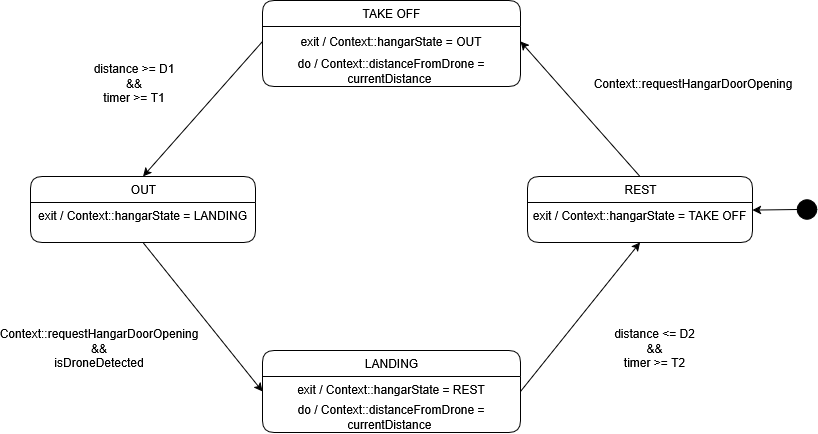
\includegraphics[width=\linewidth]{images/hangar.png}
    \caption{Macchina a stati dell'Hangar}
    \label{fig:hangar}
\end{figure}

\begin{figure}[H]
    \centering
    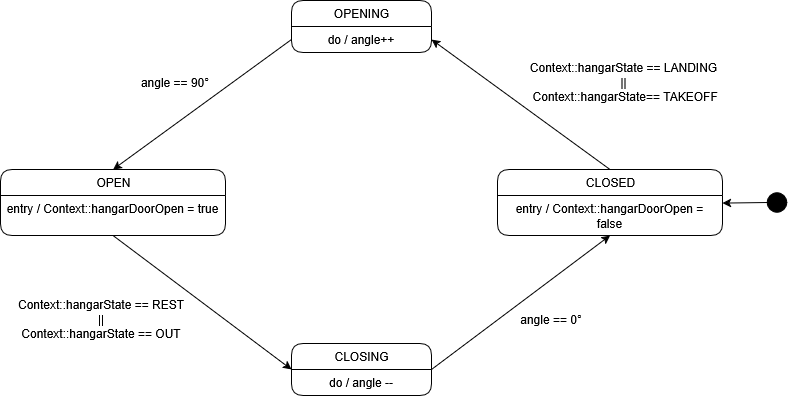
\includegraphics[width=\linewidth]{images/hangar_door.png}
    \caption{Macchina a stati della porta dell'Hangar}
    \label{fig:hangarDoor}
\end{figure}

\begin{figure}[H]
    \centering
    \vspace{50px}
    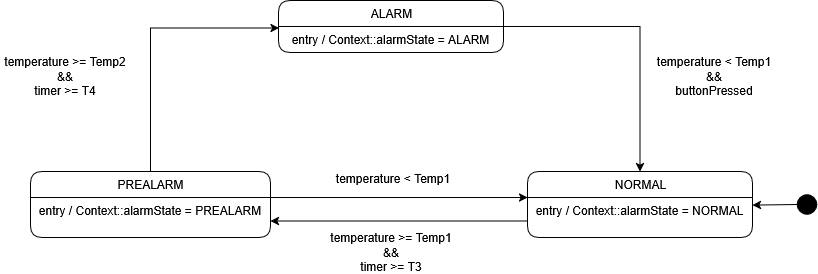
\includegraphics[width=\linewidth]{images/alarm.png}
    \caption{Macchina a stati dell'allarme}
    \label{fig:alarm}
\end{figure}

\begin{figure}[H]
    \centering
    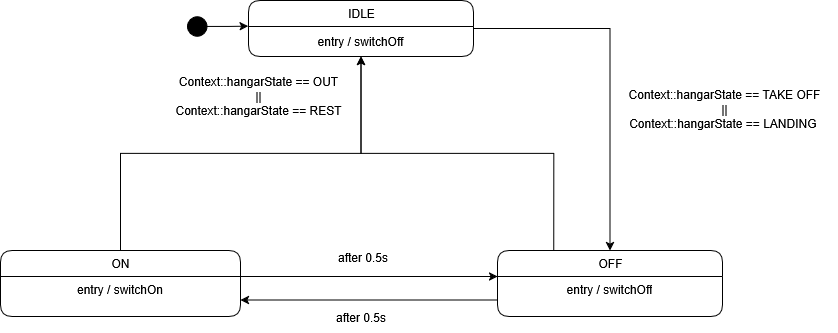
\includegraphics[width=\linewidth]{images/blinking.png}
    \caption{Macchina a stati del blinking del led}
    \label{fig:blinking}
\end{figure}

\chapter{Progettazione circuito}

\section{Schema}

\begin{figure}[H]
    \centering
    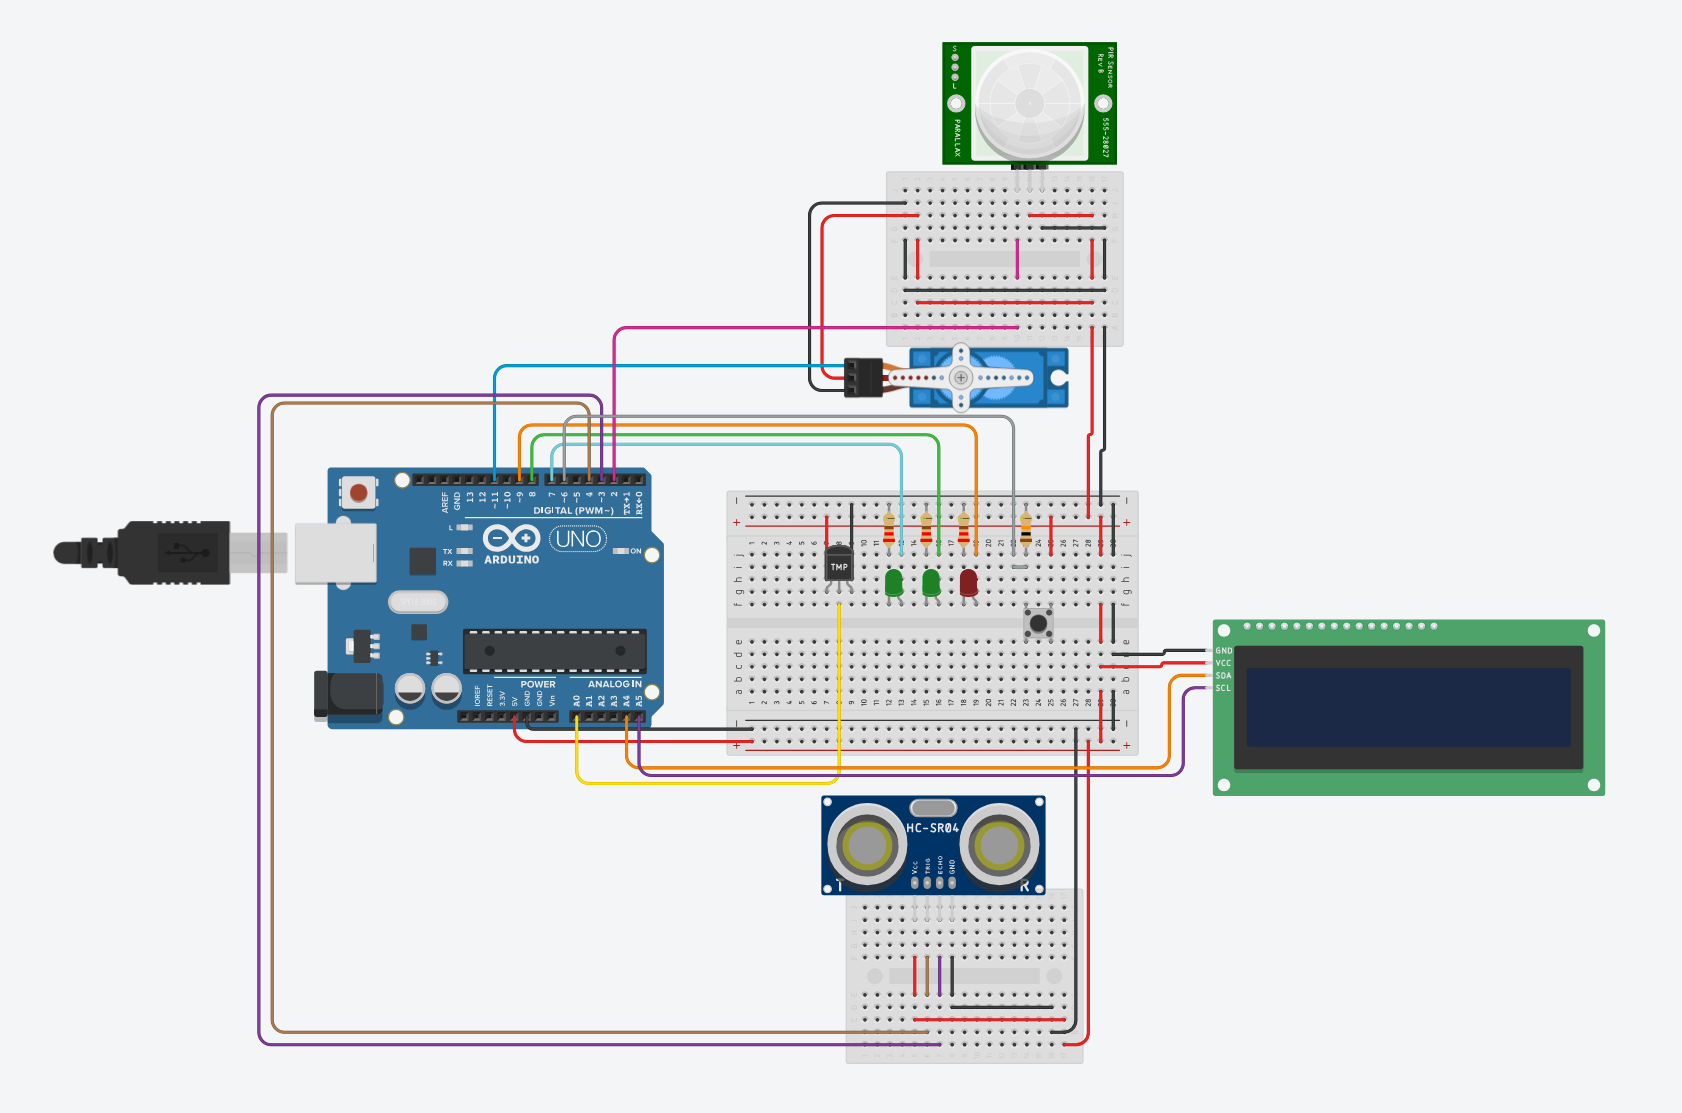
\includegraphics[width=\linewidth]{images/circuit.png}
    \caption{Schema Tinkercad rappresentante il circuito}
    \label{fig:circuit}
\end{figure}

Rispetto all'implementazione fisica, nel corrente schema si è scelto di inserire il termoresistore TMP36 poiché su Tinkercad non è presente il termistore NTC utilizzato nel progetto.

\chapter{Applicazione Java}

\section{Interfaccia grafica}
\begin{figure}[H]
    \centering
    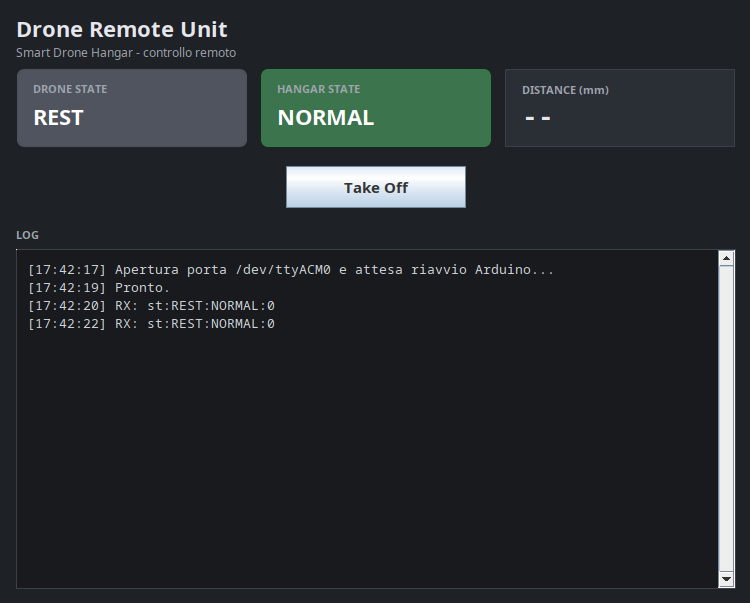
\includegraphics[width=\linewidth]{images/dru.png}
    \caption{Applicazione Drone Remote Unit}
    \label{fig:dru}
\end{figure}
\section{Comunicazione Arduino-Applicazione}

La comunicazione tra l'Arduino e la DRU avviene su una singola linea seriale a
\textbf{115200 baud}, con un protocollo testuale a righe: ogni messaggio è una
stringa che termina con un carattere di nuova riga (\texttt{\textbackslash n}),
composta da un prefisso a due lettere seguito da \texttt{:} e dal payload. La
definizione dei prefissi e delle costanti è condivisa
tra \texttt{Protocol.h} lato Arduino e \texttt{Protocol.java} lato DRU, in modo
che le due parti non possano disallinearsi.

\subsection{Messaggi Arduino → DRU}

\begin{table}[H]
\centering
\small
\begin{tabularx}{\textwidth}{|l|p{3.3cm}|X|}
\hline
\textbf{Prefisso} & \textbf{Formato} & \textbf{Descrizione} \\
\hline
\texttt{st:} &
\texttt{st:<droneState>:\linebreak <hangarState>:\linebreak <distanceCm>} &
Stato corrente, inviato periodicamente ad ogni tick di \texttt{SerialCommTask}. \\
\hline
\texttt{al:} &
\texttt{al:ALARM} &
Notifica di allarme, inviata una tantum quando l'hangar entra in stato di allarme con il drone fuori dall'hangar. \\
\hline
\texttt{lo:} &
\texttt{lo:<messaggio>} &
Messaggio diagnostico/di log, mostrato nel pannello di log della DRU (es. rilevamento del drone da parte del PIR). \\
\hline
\end{tabularx}
\caption{Messaggi inviati dall'Arduino alla DRU}
\end{table}

I campi di \texttt{st:} possono assumere i seguenti valori:
\begin{itemize}
    \item \textbf{droneState}: \texttt{REST}, \texttt{TAKEOFF}, \texttt{OUT}, \texttt{LANDING};
    \item \textbf{hangarState}: \texttt{NORMAL}, \texttt{PREALARM}, \texttt{ALARM};
    \item \textbf{distanceCm}: distanza misurata dal sonar, in centimetri;
    vale \texttt{-1} quando non è disponibile una lettura valida (drone non
    rilevato, oppure fuori dalle fasi di decollo o atterraggio).
\end{itemize}
\newpage
\subsection{Messaggi DRU → Arduino}

\begin{table}[H]
\centering
\small
\begin{tabularx}{\textwidth}{|l|p{3.3cm}|X|}
\hline
\textbf{Prefisso} & \textbf{Formato} & \textbf{Descrizione} \\
\hline
\texttt{cmd:} &
\texttt{cmd:OPEN} &
Richiesta di apertura della porta dell'hangar, inviata dalla DRU quando l'operatore simula un comando di decollo o di atterraggio del drone. \\
\hline
\end{tabularx}
\caption{Messaggi inviati dalla DRU all'Arduino}
\end{table}

Il comando \texttt{cmd:OPEN} è unico per entrambe le fasi: non è la DRU a
specificare se si tratta di un decollo o di un atterraggio, ma è l'Arduino
stesso, tramite \texttt{HangarTask}, a interpretarlo in base allo stato
corrente dell'hangar (drone dentro $\rightarrow$ richiesta di decollo, drone
fuori $\rightarrow$ richiesta di atterraggio).

\subsection{Implementazione}

Lato Arduino la comunicazione è gestita da \textbf{SerialCommTask}: ad ogni
tick legge in modo non bloccante i byte disponibili sulla seriale,
riconosce i comandi completi (terminati da \texttt{\textbackslash n}) e li
traduce in richieste sul \texttt{Context} condiviso, oltre a inviare
periodicamente lo stato corrente e, quando necessario, la notifica di
allarme. Lato DRU, \textbf{SerialCommChannel} incapsula l'accesso alla porta
seriale (tramite la libreria JSSC) esponendo un'interfaccia a messaggi
asincrona, mentre \textbf{MonitoringAgent} è il thread che consuma i
messaggi in arrivo, li instrada in base al prefisso e aggiorna di
conseguenza l'interfaccia grafica (\texttt{DroneRemoteUnitView}).

\end{document}